\section{With an oracle memory, more reads help}
\label{sec:oracle}

\subsection{Symbolic oracle}

With orthogonal oracle writing, the rank-32 shared reader M1 has $D=+92.883$ pp [92.233, 93.550] and $W=+92.872$ pp [92.208, 93.564] on confirmation seed 777001, and it also improves hop 1.  % S1
The separately trained evolving-query reader exceeds B5 by +92.892 pp [92.150, 93.542] and B3 by +85.233 pp [84.233, 86.183] on hops 2 to 3 at L4, with the same primary oracle codebook.  % S2
These contrasts support repeated, query-dependent memory use for the tested task, rather than an explanation in terms of more memory-free iterations alone.  % S1 S2

Exact one-hop-per-read timing is not an empirical result.  % S7
For the trained orthogonal M1-lin reader, hop 4 accuracy at L4 is 2.483\%, and hop 8 at L8 is zero, although some intermediate longer hops are accurate at L8.  % S7
Its hop 1 accuracy falls from 99.567\% at L1 to 96.550\% at L4 and 26.300\% at L8.  % S7
These cells reject the automatic identification of a trained reader with the aligned construction of Proposition 3; they do not refute its sufficient conditions.  % S7
The benefit of depth has to be described by hop and evaluation depth, including the short-hop losses.

Random oracle codes give a different balance.
At rank 32, M1 improves the reachable hops by +33.258 pp [32.016, 34.484] but loses 18.933 pp on hop 1, and M1-lin likewise has a positive depth effect and a large hop 1 loss.  % S6
Both conditions fail only the hop-preservation criterion.  % S6
Random oracle codes are therefore not interference-free storage, and their positive reachable-hop effect is not a full gate pass.  % S6

\begin{figure}[htbp]
\centering
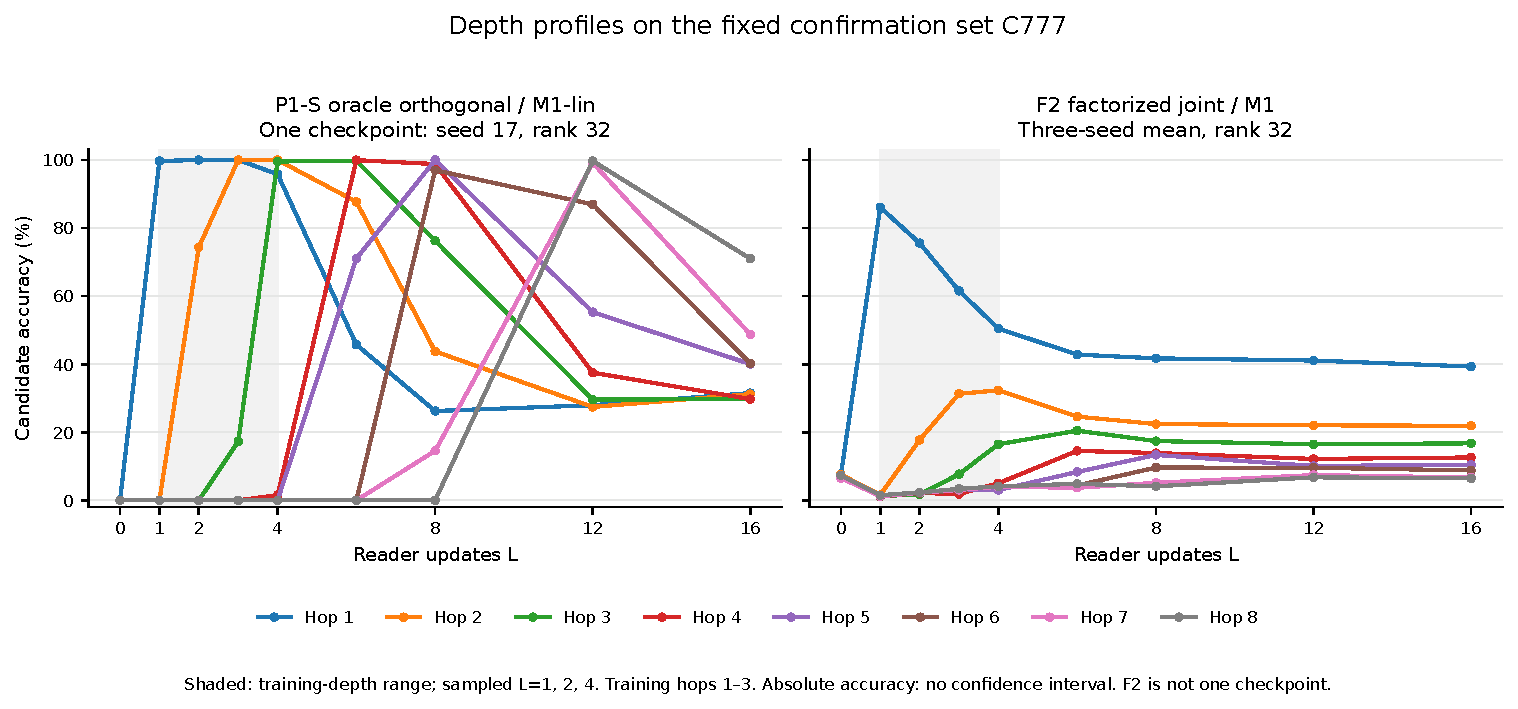
\includegraphics[width=0.96\linewidth]{quality_depth.pdf}
\caption{Quality versus evaluation depth by hop. The P1-S oracle\_orth/M1-lin curves use the individual seed-17 checkpoint; the F2 joint\_fact/M1 curves use the three-seed mean of fixed-checkpoint sweeps, because individual-checkpoint F2 cells are not committed.  % S7 S9
Candidate-restricted accuracy, confirmation seed 777001.  % S7 S9
The curves have no confidence bands and do not imply exact one-hop timing or hop preservation.  % S7 S9
}
\label{fig:qd}
\end{figure}

\subsection{Language-model oracle at two backbone sizes}
\label{sec:lm-oracle}

The language-model oracle is the registered P1-L study.
It puts the oracle memory into a frozen Qwen3 Base model and trains the question encoding and the reader and output path.
The confirmation at Qwen3-0.6B-Base used split \texttt{test}, episode indices [100000, 102000), 2,000 episodes, training seeds 17, 29 and 43, and 97.5\% paired episode-bootstrap intervals (2,000 draws) in the memory-only protocol.  % LP3
One oracle memory (oracle seed 17) is shared by every reader, and the intervals condition on the three seeds.
Only the \texttt{oracle\_random} condition ran, because the writer screens selected no learned writer.
A second confirmation (P5L) repeated the rank-128 condition at Qwen3-1.7B-Base on a range no earlier study used, \texttt{test} [104000, 106000), with the rank-128 learning rates carried over without a pilot.  % LP14

\paragraph{Memory-use check.}
Before any gate is interpreted, each reader's hop 1 EM must exceed the memory-free B3-L4@4 with a 97.5\% interval above 0 (Amendment B7).  % LP7
Table~\ref{tab:memuse} gives the result at Qwen3-0.6B-Base.
It fails at rank 32: the readers did not learn to use the oracle memory, and no claim about multiple reads in the language model is made at rank 32.
The gate outcomes there (G1-L and G2-L fail; B8@4$-$B4@1 on hops 2 to 3 is $-0.008$ pp [$-0.108$, 0.100]; M1-L4@4$-$B4@1 is $+0.058$ pp [$-0.050$, 0.167]) are reported and not interpreted.  % LP7 LP8
The check passes at rank 128 in every seed, at both backbones.  % LP7 LP14
It is a floor at hop 1 and does not show that composition uses the memory.

\begin{table}[htbp]
\centering\small
\caption{Memory-use check at Qwen3-0.6B-Base: hop 1 full-vocabulary EM, and each reader minus the memory-free B3-L4@4 in percentage points with 97.5\% intervals.  % LP7
}
\label{tab:memuse}
\begin{tabular}{@{}rp{3.0cm}p{3.0cm}p{3.4cm}p{1.5cm}p{1.9cm}@{}}
\toprule
Rank & B4@1 & B8@4 & M1-L4@4 & B3-L4@4 & Check \\
\midrule
32 & 0.067\% (+0.033 [0.000, 0.100]) & 0.067\% (+0.033 [$-0.050$, 0.133]) & 0.150\% (+0.117 [0.017, 0.233]) & 0.033\% & fails \\
128 & 19.633\% (+19.633 [18.417, 20.933]) & 19.033\% (+19.033 [17.867, 20.367]) & 47.850\% (+47.850 [46.016, 49.667]) & 0.000\% & passes, every seed \\
\bottomrule
\end{tabular}
\end{table}

\paragraph{The shared reader composes.}
On hops 2 to 3 at rank 128, the shared reader M1-L4@4 exceeds B4@1 by +21.550 pp [20.383, 22.758] (26.908\% against 5.358\%; seeds +24.450, +15.100, +25.100) with equal adapter parameter counts (475,138 each).  % LP11
This meets the Amendment-B6 criterion and is the only equal-parameter claim.
It also exceeds B5-L4@4 by +21.400 pp [20.217, 22.550] and B3-L4@4 by +26.908 pp [25.758, 27.975].  % LP11
The claim is bounded by Amendment B7: the reader learns the value-to-key lookup over the 768 seen names and composes reads inside the language model for this oracle memory; it is not equivalent to the symbolic oracle, and nothing is claimed for unseen names or entity codes, a learned writer or end-to-end use.  % LP11 LP6
\paragraph{The unshared reader B8 does not pass.}
The gated reader B8 (four unshared reads) exceeds B4@1 by only +0.983 pp [0.267, 1.717] (6.342\% against 5.358\%; seeds +0.925, +0.050, +1.975), below the registered 3 pp bar, so G1-L fails, although its hop 1 condition ($-0.600$ pp [$-1.984$, 0.767]) and its typed-replication condition (+1.550 pp [0.767, 2.367]) hold.  % LP9
B8 adds 147,456 parameters (+31.0\%) over B4.
G2-L passes (+0.833 pp [0.058, 1.550] over the fixed-query B5-L4@4 and +6.342 pp [5.758, 6.933] over the memory-free B3-L4@4), but a G2-L pass without G1-L is not a multi-read claim for B8.  % LP10
B8@4 is 20.567 pp [19.358, 21.783] below M1-L4@4 on hops 2 to 3, a secondary and ungated contrast.  % LP12
This is a difference between two architectures on one oracle memory in 17,000 steps; it is not a statement about unshared reads in general.  % LP9 LP12

\paragraph{The second backbone.}
At Qwen3-1.7B-Base the memory-use check passes in every seed: hop 1 EM exceeds the memory-free reader (0.033\%) by +30.617 pp [29.167, 32.234] for B4@1, +28.900 pp [27.517, 30.433] for B8@4 and +58.667 pp [56.983, 60.400] for M1-L4@4.  % LP14
The Amendment-B6 contrast M1-L4@4$-$B4@1 on hops 2 to 3 is +25.783 pp [24.533, 27.026] (31.958\% against 6.175\%; seeds +24.925, +26.500, +25.925), with 606,210 adapter parameters in each, so the equal-parameter result holds at a second scale of the same family.  % LP15
It has the limits of the 0.6B result, and in addition one oracle seed, three training seeds and learning rates carried without a pilot; it covers the two sizes tested and no other.  % LP15
B8@4$-$B4@1 is +1.033 pp [0.292, 1.800] (seeds +0.200, +1.725, +1.175), below the 3 pp bar, so G1-L fails again, and its hop 1 condition also fails here ($-1.717$ pp [$-3.317$, $-0.016$]) where it held at 0.6B; G2-L passes (+1.675 pp [0.908, 2.383] over B5-L4@4 and +7.167 pp [6.583, 7.758] over B3-L4@4).  % LP16 LP17
Two sizes support no scaling trend, no test across scales was registered, and the values are placed side by side without one.  % LP20

\paragraph{A copy of B8 started from the shared solution keeps it.}
G3 (B8W) tests whether a B8 reader started at the M1-L4 solution keeps that solution when its step matrices are untied.
Each M1-L4 checkpoint (Qwen3-0.6B-Base, rank 128) was copied into B8 and gave identical logits to the original in every seed (tolerance 0) before any test episode.
Then the untied copy and a continued shared M1-L4 were trained for 2,000 more steps and compared at L=4 on hops 2 to 3 of a fresh range (test [108000, 110000)).
The registered decision is that untying keeps the solution.
The untied arm minus the shared arm is +0.90 pp [0.09, 1.71] (32.40\% against 31.50\%; seeds +1.05, +0.90, +0.75), so no seed loses more than 2 pp and the pooled lower bound is above $-2$ pp.  % BW1
The shared arm moved up from its start by +5.09 pp [4.18, 6.01], so the starting reader had not converged.  % BW3
The registered wording stays: B8 has no equal-parameter status (622,594 adapter parameters against 475,138), G1-L stays failed, and nothing is said about why B8 fails from a random start.  % BW1 BW2
The untied arm is nominally above the shared arm, but the 97.5\% interval [$-0.04$, 1.81] touches 0 and no superiority test was registered, so that difference is exploratory and is not a finding.  % BW2
The result rests on one learning rate, one training length (2,000 steps), three seeds and one range, and it is sensitive to the length because the shared reference was still improving.  % BW1

\paragraph{Same-rank table.}
Table~\ref{tab:mainem} gives hop-wise EM at rank 128 for the single read B4@1 and for the two four-read readers at their trained depth.
Table~\ref{tab:maincost} gives their costs.
M1-L4 and B4 have equal parameter counts, B8 adds 147,456 parameters, and the state bytes are the persistent FP32 delta memory ($r_{\mathrm{mem}}\times r_{\mathrm{mem}}\times 4$ bytes per episode, derived from the rank and identical for the three readers, which read the same memory).  % LP23
Time per question is a measured cost, compared only within one backbone; no efficiency claim is made.  % LP13 LP19

\begin{table}[htbp]
\centering\footnotesize
\caption{Exact-match accuracy (\%) by hop at rank 128, primary setting, seed means of three training seeds, one oracle seed.  % LP23
}
\label{tab:mainem}
\gtMainEM
\end{table}

\begin{table}[htbp]
\centering\footnotesize
\caption{Costs of the same readers: parameters, persistent state, and measured time per question (memory-only protocol, batch of 16 episodes).  % LP23
}
\label{tab:maincost}
\gtMainCost
\end{table}

\paragraph{Three kinds of evidence.}
Table~\ref{tab:kinds} separates the evidence by the question it answers.
The three kinds are never pooled.

\begin{table}[htbp]
\centering\small
\caption{Three kinds of evidence.}
\label{tab:kinds}
\begin{tabular}{@{}p{2.4cm}p{3.2cm}p{7.2cm}p{1.9cm}@{}}
\toprule
Kind & Question & Result & Rows \\
\midrule
Oracle composition & Does a trained reader compose reads over a privileged memory? & M1-L4@4 exceeds B4@1 at equal parameters on hops 2 to 3 by +21.550 pp (0.6B) and +25.783 pp (1.7B); B8 fails G1-L at both backbones & LP7 to LP20 \\
Learned-writer access & Can a learned writer build that memory? & No writer reaches the 0.80 gate in any screen (best final WP-L4 arm 33.5\%; DPFP 60.8\% and 73.0\% at E=8; DPFP-X 66.2\% and 59.3\%; SQ2 best cell 72.3\%; LSQT best arm 46.1\%); each registered decision keeps the learned-writer line stopped & LL9, DP1, DP4, PD1, SQ1, LQ1 \\
Mechanism evidence & Where and how does the walk happen? & Per-step readouts are decoding only; bridge patching at the final question position shifts the answer by +0.391 pp against a 10 pp bar; final-position-only reads lower M1-L4's hops 1 to 3 EM by 29.906 pp (a distribution shift) & LP5, PC1 to PC3 \\
\bottomrule
\end{tabular}
\end{table}
% LL9 DP1 DP4 PD1 SQ1 LQ1 LP5 PC1 PC2 PC3 LP4

\subsection{Depth by hop}
\label{sec:depth-hop}

The M1-L4 checkpoint is trained at L=4 on hops 1 to 3.
Tables~\ref{tab:matrixA} and~\ref{tab:matrixB} evaluate that same checkpoint at depths L=1 to 8 on hops 1 to 8.
The best depth of each hop is in bold.
The last row, the oracle stop, takes the best depth for each hop using the label; it is an upper bound and a maximum over eight noisy cells, not a stopping rule.  % LP21

\begin{table}[htbp]
\centering\footnotesize
\caption{Qwen3-0.6B-Base: seed-mean EM (\%) of the M1-L4 checkpoint by evaluation depth $L$ and hop (primary setting, rank 128). The last row gives the best depth in parentheses.  % LP21
}
\label{tab:matrixA}
\gtMatrixSmall
\end{table}

\begin{table}[htbp]
\centering\footnotesize
\caption{Qwen3-1.7B-Base: the same matrix.  % LP21
}
\label{tab:matrixB}
\gtMatrixLarge
\end{table}

At the trained depth the reader reaches hop 3.
At L=4 its EM on hops 1 to 3 is 47.9/35.4/18.5\% at 0.6B and 58.7/41.5/22.5\% at 1.7B.
On hops 5 to 8 it is 3.9 to 5.0\% and 3.1 to 3.9\%, not above the single read B4@1 (5.0 to 5.8\% and 5.5 to 5.7\% on hops 4 to 8).  % LP21
The same checkpoint reaches hops 4 to 8 at 9.9 to 16.6\% (0.6B) and 9.8 to 20.9\% (1.7B) when run deeper.
Hop 4 peaks at L=6, and hops 5 to 8 peak at L=8, the largest depth evaluated, so their best depth is not located.
Over the same range hop 1 is lost: at L=8 it is 19.0\% and 24.1\%, against 47.9\% and 58.7\% at L=4 and 64.2\% and 77.6\% at L=2.  % LP21
These cells are at hops and depths that were never trained, they carry no interval, and they rest on one oracle seed and three training seeds.
The paper does not say that the reader cannot go beyond hop 3, and it does not say that the reader composes up to hop 8.
A label-free stop is evaluated in Section~\ref{sec:stop}.

\subsection{A label-free stop at inference}
\label{sec:stop}

The matrix suggests that the depth that suits a hop grows with the hop, and that the deployed depth L=4 is a compromise.
LSR (G2) asks whether a per-question stop that uses no label can raise hops 4 to 8 over fixed L=4 without a large loss on hop 1.
It evaluates the six rank-128 M1-L4 checkpoints (three seeds at each backbone) and trains nothing.
Three rules were registered: R1 stops when the relative change of the state falls below a threshold, R3 when the norm of the read, relative to the first read, falls below a threshold, and R2 when the model's top-1 answer has not changed over two consecutive depths (no parameter).
The thresholds of R1 and R3 were chosen on validation episodes under a hop-1 constraint, and the registered comparisons use the test range [106000, 108000) with 99.17\% intervals for six comparisons.  % LS1

\paragraph{R1 and R3 had no feasible threshold.}
At both backbones no value of the 25-value validation grid kept the hop-1 loss against fixed L=4 within the registered margin (8 pp pooled, 10 pp per seed), so no test statistic was computed.
The traces show why.
At 0.6B the read norm relative to the first read never falls below 1 (median 1.0 to 1.1), so a threshold below 1 never fires and one above 1 stops at the first step.
At 1.7B it grows to about 10 and the relative change of the state stays at 0.5 to 0.7, so both rules stop at the first step or run to depth 8.
This does not show that no other label-free signal works.  % LS2

\paragraph{R2 raises hops 4 to 8 over fixed L=4.}
Against fixed L=4, which is also the best fixed depth under the validation constraint, the R2 stop raises hops 4 to 8 by +3.90 pp [3.35, 4.43] at 0.6B and +5.68 pp [5.09, 6.25] at 1.7B, in every seed (+4.58, +3.25, +3.87 and +5.46, +5.71, +5.86), and it raises hop 1 by +6.28 and +4.70 pp.
So a label-free per-question stop raised hops 4 to 8 over fixed L=4 at both scales, in the oracle-memory condition, evaluation only.  % LS1
The result comes with its costs.
Hop 2 falls by 10.83 pp [$-11.85$, $-9.87$] at 0.6B and by 12.27 pp [$-13.32$, $-11.23$] at 1.7B, and hop 3 by 3.28 and 3.65 pp, so R2 does not improve every hop.
On hops 4 to 8 it stays below fixed L=8 ($-3.54$ and $-5.05$ pp), and it recovers about half of the headroom between L=4 and the best fixed depth for each hop.
It reads 5.60 and 5.66 times per question against 4, and each stopping decision needs a pass through the frozen upper layers, so a question that stops after $s^{*}$ reads needs $s^{*}+1$ such passes (6.60 and 6.66 on average).
R2 was not timed, and no efficiency or latency claim is made.  % LS3
The stop depends only weakly on the hop: the mean number of reads rises from 4.97 at hop 1 to 5.86 at hop 8 at 0.6B, and from 4.87 to 5.93 at 1.7B.  % LS3
Table~\ref{tab:lsr} puts the R2 row next to the fixed-depth rows.
The LSR range differs from the range of the matrices above, so its L=4 cells differ slightly from them (hop 1 is 48.0\% here and 47.9\% there), and the two are not pooled.  % LS4
The intervals condition on three training seeds per backbone and one oracle code table.

\lsrtable
% LS4

\subsection{Seed-level statistics}
\label{sec:seeds}

The registered intervals resample episodes and hold the three fitted seeds fixed.
Tables~\ref{tab:seedsA} and~\ref{tab:seedsB} print the three seed effects of each headline contrast beside a seed-level interval.
The seed-level interval is the mean of the three seed effects plus or minus $t(0.9875;2)=6.205$ times their sample standard error, the two-sided 97.5\% level of the registered intervals.  % LP22
Both kinds of interval are conditional on three fitted seeds and one fixed oracle code table (oracle seed 17, one layout).
Neither covers future training seeds or other code tables, and the $t$-interval treats the three seed effects as exchangeable draws, which three values cannot test.

\begin{table}[htbp]
\centering\footnotesize
\caption{Qwen3-0.6B-Base: seed effects and intervals for the headline contrasts at rank 128 (pp).  % LP22
}
\label{tab:seedsA}
\gtSeedsSmall
\end{table}

\begin{table}[htbp]
\centering\footnotesize
\caption{Qwen3-1.7B-Base: the same contrasts.  % LP22
}
\label{tab:seedsB}
\gtSeedsLarge
\end{table}

The seed-level interval excludes 0 for the B6 contrast (M1-L4@4$-$B4@1) and for G2-L against the memory-free reader, at both backbones.
It includes 0 for the G1-L contrasts and for G2-L against the fixed-query reader at both backbones, so the G2-L pass over B5-L4@4 is a statement about the fitted seeds.
The registered decisions use the episode intervals and are unchanged.  % LP22
